%appendix blhablhaakljfdldskj
%Created MB 03-01

\section{Muon Mass Calibration}

For heavy ($\mu$ and heavier) charged particles passing through
matter, the amount of energy deposited depends on the incident
momentum of the particle. The relationship is given by the Bethe-Block
equation \cite{yao}:

\begin{equation}
-\frac{dE}{dx} = Kz^2\frac{Z}{A}\frac{1}{\beta^2}\left[\frac{1}{2}ln\frac{2m_ec^2\beta^2\gamma^2T_max}{I} - \beta^2 - \frac{\delta(\beta\gamma)}{2}\right]
\end{equation}

where $\beta = v/c$ and $\gamma = 1/\sqrt{1 - \frac{v_{\mu}^2}{c^2}}$
are of the incoming particle, and the other parameters are constants
or properties of the material.

The rates of mean energy loss of muons for a range of incident momenta
are shown in Figure~\ref{figure:dEdx} \cite{yao}. The minimum
ionization energies vary with material; in our experiment, the
scintillator consisted of polystyrene ($C_8H_9$). The minumum
ionization energy was determined by weighing the $C$ and $H$ values,
$1.75\pm 0.1$ MeV g$^{-1}$cm$^{2}$ and $4.0\pm 0.1$
MeV g$^{-1}$cm$^{2}$, respectively, according to the mass ratio of the
two elements in the compound, to give a the energy deposited by a
minimum-ionizing muon to be $1.85 \pm 0.1$ MeV g$^{-1}$cm$^{2}$ in the
scintillator material.

\label{energy_loss}
\begin{figure}[h]
\begin{center}
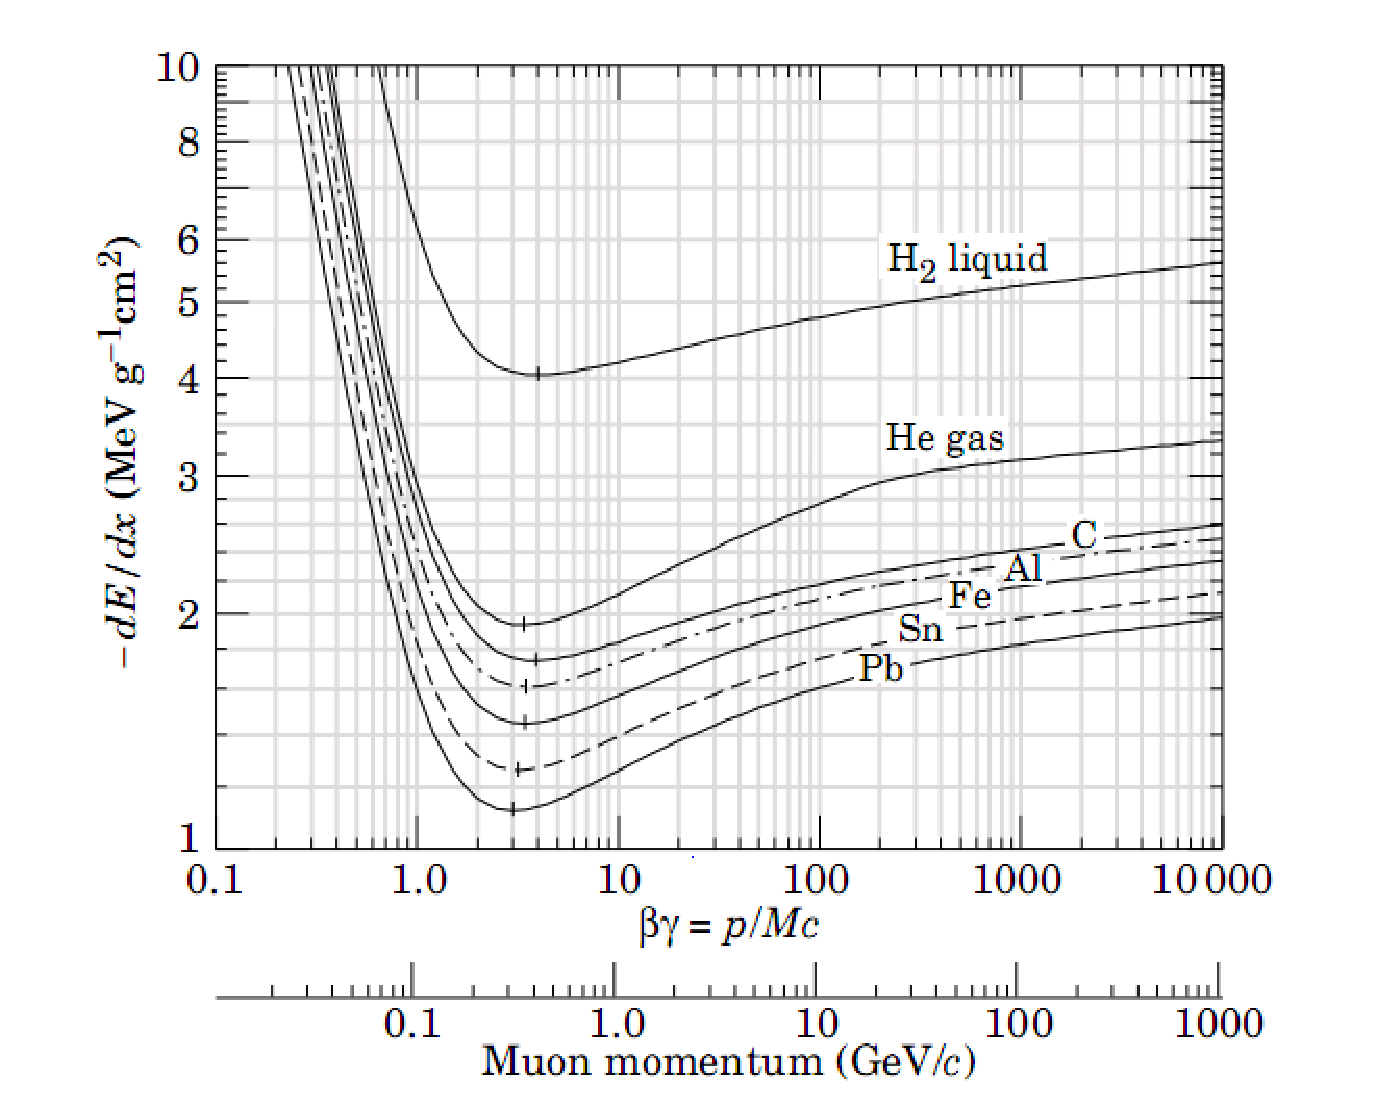
\includegraphics[width = 130mm]{figures/energy_loss.eps}
\caption{\small{Mean energy loss in various materials \cite{yao.}}}
\label{figure:dEdx}
\end{center}
\end{figure}


